\section{Ablation studies}
\label{sec:ablations}

% Remaster, 3 October 2026.  Every factor the paper varies, one subsection
% each, summarised in Figure~\ref{fig:ablations}.  Each subsection ends with
% a one-sentence Finding.

Section~\ref{sec:results} compared the harnesses as shipped. This section
removes one factor at a time and measures what it was worth.
Figure~\ref{fig:ablations} summarises every ablation on two axes: the
paired difference in mean normalised score over the eight TabReD tasks, and
the share of trials that ended without a submission. Table~\ref{tab:grid}
and Table~\ref{tab:kdiscterm} give the per-task and per-cell numbers.

\begin{figure*}[t]
\centering
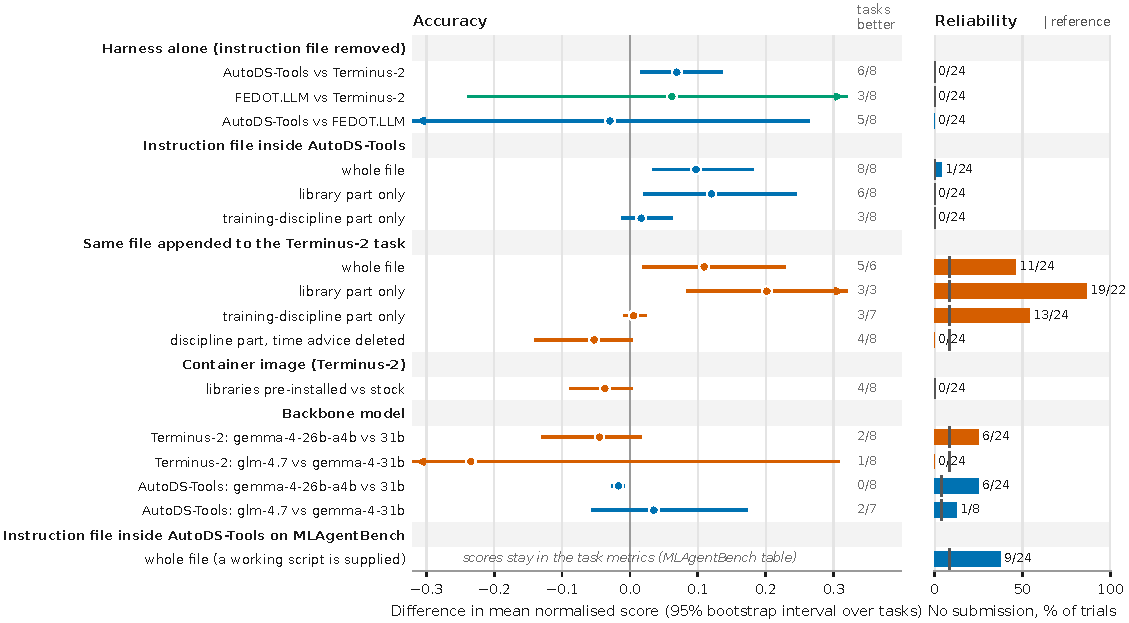
\includegraphics[width=\textwidth]{figures/fig_ablations.pdf}
\caption{Every factor the paper varies. Left: paired difference in mean
normalised score on TabReD (first configuration minus second), with the
95\% bootstrap interval over tasks and the number of tasks on which the
first is better. Right: trials that ended without a submission, with the
reference configuration as a tick. Arrows mark intervals that leave the
axis.}
\label{fig:ablations}
\end{figure*}

\subsection{Harness alone: the instruction file removed}
\label{sec:abl-harness}

With the instruction file switched off, AutoDS-Tools scores $\nAutoDSOff$
on the normalised scale, between Terminus-2 ($\nTerminus$) and FEDOT.LLM
($\nFedot$). On the same image, AutoDS-Tools without the file is ahead of
Terminus-2 on \starchAutoDSvsTerminusWins{} of 8 tasks by
$\starchAutoDSvsTerminusDiff$ (interval $\starchAutoDSvsTerminusLo$ to
$\starchAutoDSvsTerminusHi$, $p=\starchAutoDSvsTerminusP$): a small and
consistent lead that does not reach significance. FEDOT.LLM is level with
Terminus-2 on average ($p=\stshipFedotvsTerminusP$) and differs from it on
single tasks in both directions, from $+1.46$ on \texttt{ecom-offers} to
$-0.38$ on \texttt{cooking-time}.

\paragraph{Finding 5} Without the instruction file, the mean scores of the
three harnesses are close and no pairwise difference reaches $p<0.05$. The
harnesses still behave differently task by task: AutoDS-Tools is slightly
and consistently ahead of Terminus-2, and FEDOT.LLM varies most.

\subsection{The instruction file inside AutoDS-Tools}
\label{sec:abl-file}

Table~\ref{tab:grid} crosses the two parts of the file on AutoDS-Tools: four
cells of 24 trials on one image, one machine and one concurrency setting,
differing in the instruction file and in nothing else. The whole file lifts
the normalised score from $\nAutoDSOff$ to $\nAutoDS$, improving all eight
tasks ($\stfileBothDiff$, interval $\stfileBothLo$ to $\stfileBothHi$,
$p=\stfileBothP$). The library instruction alone lifts it to $\nGridTool$
(\stfileToolWins{} of 8 tasks, $p=\stfileToolP$), on par with tuned
XGBoost ($\sttoolVsXGBDiff$, $p=\sttoolVsXGBP$) and the best cell in the
paper; adding the discipline instruction on top changes it by
$\stbothVsToolDiff$ ($p=\stbothVsToolP$). The discipline instruction alone
lifts it to $\nGridDisc$ (\stfileDiscWins{} of 8, $p=\stfileDiscP$).
The traces show what the library instruction changes: with it,
AutoDS-Tools calls LightAutoML~\citep{vakhrushev2021lightautoml} in all 24
trials of both cells, and without it writes LightGBM, XGBoost or CatBoost by
hand in all 24 trials of both cells (Section~\ref{sec:spontaneous}). In the task metrics the library instruction improves the
mean by $\gridToolMeanU\%$, the discipline instruction by
$\gridDiscMeanU\%$ and both together by $\gridBothMeanU\%$, below the
$\gridSumHalvesU\%$ sum of the two. Two tasks carry most of the library
effect, \texttt{ecom-offers} ($\gridToolEcom\%$) and
\texttt{homecredit-default} ($\gridToolHomecredit\%$); no other task moves
by more than $\gridToolRestMax\%$. Of the $\gapAgentsShip$ by which
AutoDS-Tools as shipped leads Terminus-2, $\layerWorthNorm$ is therefore the
file and $\gapAgentsOff$ the harness.
\begin{table*}[t]
\centering
\caption{The prescribed-knowledge layer split into its halves on AutoDS-Tools over TabReD, twenty-four trials per cell on one image and one machine. The untreated cell is given in the task's own units; the other three as relative change against it, positive is better.}
\label{tab:grid}
\small
\setlength{\tabcolsep}{5pt}
\begin{tabular}{llrrrr}
\toprule
 & & untreated & \multicolumn{3}{c}{change against untreated, \%} \\
\cmidrule(l){4-6}
Task & Metric & cell & $K_{\text{tool}}$ only & $K_{\text{disc}}$ only & both \\
\midrule
\texttt{homesite-insurance} & ROC-AUC & 0.9600 & +0.10 & -0.03 & +0.12 \\
\texttt{ecom-offers} & ROC-AUC & 0.5649 & +3.68 & +1.24 & +2.67 \\
\texttt{homecredit-default} & ROC-AUC & 0.8559 & +0.79 & +0.20 & +0.86 \\
\texttt{sberbank-housing} & RMSE & 0.2516 & -0.31 & 0.00 & +0.07 \\
\texttt{cooking-time} & RMSE & 0.4835 & +0.47 & -0.04 & +0.30 \\
\texttt{delivery-eta} & RMSE & 0.5476 & 0.00 & -0.05 & +0.04 \\
\texttt{maps-routing} & RMSE & 0.1627 & +0.64 & +0.09 & +0.45 \\
\texttt{weather} & RMSE & 1.4968 & +0.14 & -0.41 & +1.24 \\
\midrule
mean over tasks & & & +0.69 & +0.12 & +0.72 \\
tasks improved & & & 6 of 8 & 3 of 8 & 8 of 8 \\
\bottomrule
\end{tabular}
\end{table*}


The two parts also cost differently. Naming the library shortens the
agent's search and lengthens the fit: the median trial goes from
$\gridNeitherMin$ minutes without instructions to $\gridToolMin$ with the
library named, and the API cost per trial falls from $\gridNeitherCost$ to
$\gridToolCost$ dollars. The discipline instruction does the opposite,
adding $\gridDiscCostPct\%$ to the cost and cutting the median trial to
$\gridDiscMin$ minutes. No cell lost more than one trial of 24.

\paragraph{Finding 6} Inside AutoDS-Tools the instruction file improves all
eight TabReD tasks ($p=\stfileBothP$) and accounts for $\layerWorthNorm$ of
the $\gapAgentsShip$ lead over Terminus-2. The library instruction carries
the effect by handing the modelling to LightAutoML, and alone reaches the
level of tuned XGBoost; the two parts gain less together than the sum of
their separate gains.

\subsection{The same file inside Terminus-2}
\label{sec:abl-terminus}

The file is composed on the host and reaches only its own agent, so to test
it in a second harness we appended the byte-identical parts to the
Terminus-2 task statement and ran 24 trials per cell on one machine, image,
backbone and concurrency setting (Table~\ref{tab:kdiscterm}); the part that
should be present appears in every trajectory, the part that should be
absent in none. Accuracy does not move: in the discipline cell every value
lands inside the spread of the cell without instructions, and the mean
difference is $\sttermDiscDiff$ (interval $\sttermDiscLo$ to
$\sttermDiscHi$). What moves is whether a trial produces an answer. Trials
ending without a submission go from \ktNeitherLost{} of 24 without
instructions to \ktDiscLost{} with the discipline instruction
($p=\ktPDiscVsNeither$), \ktToolLost{} of \ktToolTrials{} with the library
instruction ($p=\ktPToolVsNeither$) and \ktBothLost{} of 24 with both. None
is a timeout. The agent launches a fit in the foreground, sees a terminal
that has stopped producing output because its own job holds it, concludes
that reporting is broken and marks the task complete.
\begin{table}[t]
\centering
\caption{The instruction file appended to the Terminus-2 task statement on the eight TabReD tasks, 24 trials per cell on one machine, image and language model. Lost: trials ending with no submission. Steps and minutes are medians per trial.}
\label{tab:kdiscterm}
\footnotesize
\setlength{\tabcolsep}{3pt}
\begin{tabular}{lrrrrrrr}
\toprule
Cell & Trials & Lost & Tasks & Steps & Min & \$/trial & rel.\ \% \\
\midrule
none & 24 & 2 & 8/8 & 6 & 2.5 & 0.0029 & ref. \\
discipline & 24 & 13 & 7/8 & 18 & 14.1 & 0.0303 & -0.05 \\
discipline trimmed & 24 & 0 & 8/8 & 7 & 3.0 & 0.0044 & -0.69 \\
library & 22 & 19 & 3/8 & 14 & 10.2 & 0.0107 & +1.21 \\
both & 24 & 11 & 6/8 & 20 & 18.4 & 0.1172 & +1.13 \\
\bottomrule
\end{tabular}
\par\smallskip
\begin{minipage}{0.97\linewidth}\scriptsize The library cell lost two trials to a network fault and reports twenty-two. No cell had a timeout. Tasks: how many of eight returned a metric at least once. rel.\ \%: mean relative change against the cell without the file over the tasks that cell returns; the last two rows average over a surviving minority. Fisher's exact test on lost trials, two-sided: discipline against none $p=0.0013$; trimmed against discipline $p=2.6\times10^{-5}$; trimmed against none $p=0.49$; library against none $p=9.6\times10^{-8}$; library against both $p=0.0055$; a Holm correction changes no conclusion. Trimmed: the discipline instruction with its two paragraphs about training time removed.\end{minipage}
\end{table}


Two of the seven sections of the discipline instruction cause this. One
offers a hundred epochs as a starting budget and tells the agent to raise
it; the other tells it to assume it has ``hours, not minutes'' and that a
training phase finishing ``within a couple of minutes'' signals
undertraining. The median trial without instructions is two and a half
minutes of gradient-boosted trees and is not undertrained; the text was
written for convolutional and encoder models. Deleting those two sections
and keeping the other five loses no trial of 24, against \ktDiscLost{} with
the full instruction ($p=\ktPTrimVsDisc$) and \ktNeitherLost{} with none
($p=\ktPTrimVsNeither$), and returns the median trial to three minutes. With
the library instruction the fit is long because the prescribed library is
slow, and there the discipline instruction protects: the library instruction
alone loses \ktToolLost{} of \ktToolTrials{} trials, both together
\ktBothLost{} of 24 ($p=\ktPToolVsBoth$), because the discipline text tells
the agent that a long-running job is normal. AutoDS-Tools met none of this:
the same four cells inside its own harness lost none, none, none and one
trial of 24 (Section~\ref{sec:abl-file}).

\paragraph{Finding 7} Appended to Terminus-2, the file leaves accuracy
unchanged and ends \ktDiscLost{} of 24 trials without a submission with its
discipline part, \ktToolLost{} of \ktToolTrials{} with its library part and
\ktBothLost{} of 24 with both. For the discipline part, deleting two
paragraphs about training time restores every trial. The effect of an
instruction file has to be measured in each harness separately.

\subsection{The same file from a working script}
\label{sec:abl-script}

The two AutoDS-Tools column groups of Table~\ref{tab:mlab} ablate the whole
file over MLAgentBench, where every task starts from a working script. The
costly side is unambiguous: on \texttt{clrs}, \texttt{fathomnet} and
\texttt{feedback} the cell without the file scores in every attempt
($\mlabClrsOff$ pointer accuracy, $\mlabFathomnetOff$ micro-F1,
$\mlabFeedbackOff$ MCRMSE), and the cell with the file submits nothing in
any attempt, every attempt exhausting the task's agent budget. The paying
side is thin: only \texttt{ogbn-arxiv} gains by a margin that clears the
spread of either cell ($\mlabOgbnOff$ to $\mlabOgbnOn$);
\texttt{spaceship-titanic} and \texttt{house-price} do not differ beyond
their spreads, and \texttt{amp-parkinsons} moves against the file. The file
replaces a decision that the supplied script had already made, and on
MLAgentBench that replacement leaves no submission on \mlabWiped{} of
\mlabRepeated{} tasks and improves one.

The two benchmarks differ in tasks, metrics and budgets as well as in
starting point, so this is one factor observed across two protocols and we
do not add the win counts. The claim that holds inside each protocol is
this: from scratch, the file improves every TabReD task and loses no trial;
from a working script, it loses every attempt on \mlabWiped{} of
\mlabRepeated{} tasks.

\paragraph{Finding 8} The file that improves every TabReD task leaves no
submission on \mlabWiped{} of \mlabRepeated{} MLAgentBench tasks and helps
on one; what differs is whether a working default was already in place. The
count is a lower bound on the cost of the file, since the repair loop of
AutoDS-Tools absorbs part of it (Section~\ref{sec:friction}).

\subsection{Container image}
\label{sec:abl-image}

Running Terminus-2 on the enriched image built for AutoDS-Tools, same
tasks and three attempts each, changes the mean normalised score by
$\stimageDiff$ (interval $\stimageLo$ to $\stimageHi$,
$p=\stimageP$); \matchedWithin{} of the eight tasks stay inside the
harness's own noise floor, and the one outside it,
\texttt{sberbank-housing}, is one attempt that trained a thousand boosting
rounds without early stopping. Across all 24 trials the agent named none of
the three libraries the image pre-installs and went to gradient boosting by
hand, as on the stock image, where it had installed LightGBM itself. A
pre-installed library therefore changes the result only when an instruction
names it.

\paragraph{Finding 9} Pre-installing libraries that no instruction names
changes the mean normalised score by $\stimageDiff$, inside the noise of the
harness, and the agent uses none of them.

\subsection{Backbone}
\label{sec:abl-backbone}

Swapping the backbone under each harness, with tasks, image and instructions
unchanged, changes accuracy by less than the instruction file and changes
reliability by more. Under AutoDS-Tools
the smaller \texttt{gemma-4-26b-a4b} changes the normalised score by
$\stautodsSmallDiff$, worse on all eight tasks and by under one per cent in
the task metrics, and \texttt{glm-4.7} changes it by $\stautodsBigDiff$ (interval
$\stautodsBigLo$ to $\stautodsBigHi$, seven tasks scored). Under Terminus-2
the smaller model gives $\sttermSmallDiff$ and \texttt{glm-4.7}
$\sttermBigDiff$, the latter through one task: on \texttt{sberbank-housing}
the stronger model left the gradient-boosting default for a random forest
and lost $46\%$ of RMSE. On \texttt{ecom-offers} the same departure
produced the best ROC-AUC of any agent in this paper, $0.627$. Across the
same rows the price of a sweep of 24 trials varies \axPriceSpread$\times$,
from \$0.07 to \$0.93 under Terminus-2. Reliability moves in
opposite directions for the two harnesses: under Terminus-2 trials without
a submission fall from \axTerminusSmallLost{} of 24 to
\axTerminusRefLost{} to \axTerminusBigLost{} as the backbone strengthens;
under AutoDS-Tools they are lowest at the model the system was built
against (\axAutoDSRefLost{} of 24) and rise on both sides
(\axAutoDSSmallLost{} of 24 and \axAutoDSBigLost{} of the
\axAutoDSBigTrials{} trials we could afford), because a stronger model makes
the six agents exchange more text inside the same hour and more trials reach
the ceiling. Two models one generation older, \texttt{gemma-3-12b-it} and
\texttt{gemma-3-27b-it}, returned no usable submission in smoke trials on
\texttt{cooking-time} (the smaller emitted tool calls with empty arguments,
the larger left its submission in the wrong directory). There is a
capability floor below which neither harness produces a usable submission.

\paragraph{Finding 10} A backbone swap that changes the API cost
\axPriceSpread$\times$ moves accuracy by $\stautodsSmallDiff$ to
$\stautodsBigDiff$ under AutoDS-Tools and, under Terminus-2, by up to
$\sttermBigDiff$ through a single task; it moves reliability in opposite
directions for the two harnesses.
